\documentclass[fleqn,10pt]{wlscirep}
\usepackage[utf8]{inputenc}
\usepackage[T1]{fontenc}
\title{Preliminary Comparison of CRISPR/Cas9-based Screening Data Analysis Algorithms}

\author[1,*]{Y.Q. Yang}

\begin{abstract}
In the opening report of CRISPR/Cas9-based Screening Data Analysis, I introduced MAGeCK and BAGEL, which are both CRISPR/Cas9-based screening data analysis algorithms that can be applied for essential gene identification.  However, I only summarized the principles of two algorithms, but did not explicitly compare the difference between them in all aspects.  Therefore, I added detailed comparison information in this report, and preliminary process the screening data given by Professor Wang. Due to lack of time as well as corresponding data, the screening data were only calculated via MAGeCK.
\end{abstract}
\begin{document}

\flushbottom
\maketitle

\thispagestyle{empty}

\section*{Background}

MAGeCK and BAGEL are two known tools that have been specifically designed for CRISPR/CAS9-based essential gene identification. In order to find out which relatively performs better, I have to compare them from both their detailed algorithms in different steps and the actual analysis results obtained from on our own reserach data.  According to the above requirements, I generally planned my project workflow as below:

\begin{itemize}
    \item (1) Compare the principle of screening data analysis between two methods in all aspects(listed in order):
        \subitem read count calculation;
        \subitem read count normalization;
        \subitem sgRNA ranking(not exist in BAGEL, which will be explained later);
        \subitem essential gene ranking;
    \item (2) Rank sgRNA and identify essential genes via two methods based on absolutely the same screening data.
    \item (3) Identify enriched pathway via MAGeCK only since this function is not inclued in BAGEL.
    \item (4) Compare MAGeCK with other pathway analysis tools and find out which one does a better job.
    \item (5) Summarize the tools that perform well at each step, improve the deficiencies, and thus generating a new workflow for CRISPR/Cas9-based essential gene and enriched pathway identification.
    \end{itemize}

\section*{Results}

\subsection*{Step-by-step principle comparison between MAGeCK}

Example text under a subsection. Bulleted lists may be used where appropriate, e.g.


\subsubsection*{Third-level section}
 
Topical subheadings are allowed.

\section*{Discussion}

The Discussion should be succinct and must not contain subheadings.

\section*{Methods}

Topical subheadings are allowed. Authors must ensure that their Methods section includes adequate experimental and characterization data necessary for others in the field to reproduce their work.

\bibliography{sample}

\noindent LaTeX formats citations and references automatically using the bibliography records in your .bib file, which you can edit via the project menu. Use the cite command for an inline citation, e.g.  \cite{Hao:gidmaps:2014}.

For data citations of datasets uploaded to e.g. \emph{figshare}, please use the \verb|howpublished| option in the bib entry to specify the platform and the link, as in the \verb|Hao:gidmaps:2014| example in the sample bibliography file.

\section*{Acknowledgements (not compulsory)}

Acknowledgements should be brief, and should not include thanks to anonymous referees and editors, or effusive comments. Grant or contribution numbers may be acknowledged.

\section*{Author contributions statement}

Must include all authors, identified by initials, for example:
A.A. conceived the experiment(s),  A.A. and B.A. conducted the experiment(s), C.A. and D.A. analysed the results.  All authors reviewed the manuscript. 

\section*{Additional information}

To include, in this order: \textbf{Accession codes} (where applicable); \textbf{Competing interests} (mandatory statement). 

The corresponding author is responsible for submitting a \href{http://www.nature.com/srep/policies/index.html#competing}{competing interests statement} on behalf of all authors of the paper. This statement must be included in the submitted article file.

\begin{figure}[ht]
\centering
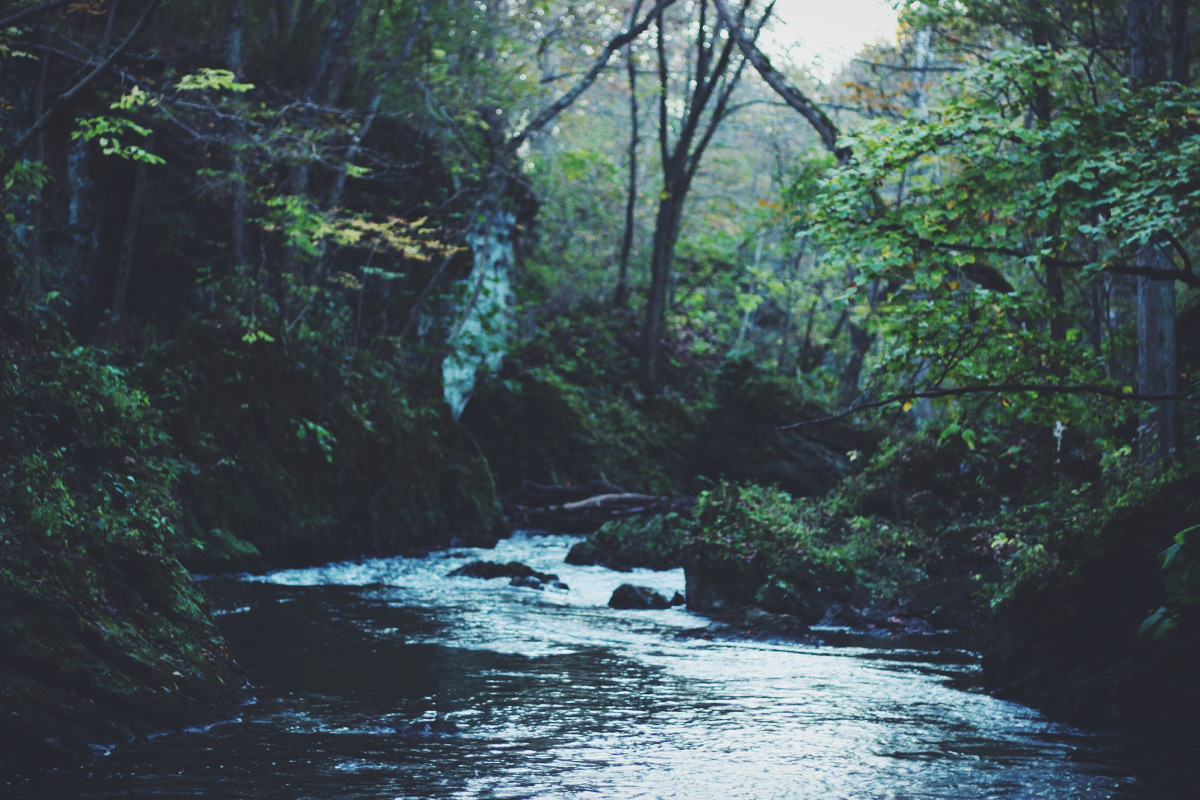
\includegraphics[width=\linewidth]{stream}
\caption{Legend (350 words max). Example legend text.}
\label{fig:stream}
\end{figure}

\begin{table}[ht]
\centering
\begin{tabular}{|l|l|l|}
\hline
Condition & n & p \\
\hline
A & 5 & 0.1 \\
\hline
B & 10 & 0.01 \\
\hline
\end{tabular}
\caption{\label{tab:example}Legend (350 words max). Example legend text.}
\end{table}

Figures and tables can be referenced in LaTeX using the ref command, e.g. Figure \ref{fig:stream} and Table \ref{tab:example}.

\end{document}